\documentclass[12pt,a4paper]{article}
\usepackage[utf8]{inputenc}
\usepackage[T1]{fontenc}
\usepackage{times}                   % Font: Times New Roman
\usepackage[margin=2.54cm]{geometry} % Margins: 2.54cm
\usepackage{setspace}
\singlespacing                       % Line Spacing: Single Line
\usepackage{indentfirst}             % Indent first paragraph
\usepackage{graphicx}                % Insert images
\usepackage{caption}                 % Caption formatting
\usepackage{booktabs}
\usepackage{array}
\usepackage{multirow}
\usepackage{tabularx}
\usepackage{algorithm}
\usepackage{algpseudocode}
\usepackage{listings}
\usepackage{url}
\usepackage{hyperref}
\hypersetup{colorlinks=true,linkcolor=blue,citecolor=blue,urlcolor=blue}
\lstset{
    breaklines=true,
    breakatwhitespace=false,
    basicstyle=\ttfamily\small,
    frame=single,
    numbers=left,
    numberstyle=\tiny,
    xleftmargin=2em,
    xrightmargin=2em
}
\usepackage[backend=biber,style=ieee]{biblatex}
\addbibresource{sample.bib}

\begin{document}

% =========================================================
% Cover Page
% =========================================================
\begin{titlepage}
    \centering
    \vspace*{2cm}
    {\Huge\bfseries 1st Interim Report\par}
    \vspace{2cm}

    {\huge Cross-Chain Tracing-Based Cryptocurrency Anti-Money Laundering Risk Identification System\par}

    \vfill

    {\large \textbf{Student Name:} Tang Tianhao\par}
    \vspace{0.5cm}
    {\large \textbf{Student Number:} 59720490\par}
    \vspace{1.5cm}
    {\large \textbf{Supervisor Name:} Prof LU Zhenliang\par}
    \vspace{1.5cm}
\end{titlepage}

\newpage
\tableofcontents
\thispagestyle{empty}
\newpage
\clearpage
\setcounter{page}{1}

% =========================================================
\section{Introduction}
% =========================================================

\subsection{Cryptocurrency Money Laundering at Scale}

The decentralized, pseudonymous, and globally accessible nature of blockchain has made it a significant channel for illicit fund flows alongside financial innovation. According to Chainalysis's \textit{2024 Crypto Money Laundering Report}~\cite{chainalysis2024}, illegal cryptocurrency addresses received approximately \textbf{\$40.9~billion} in 2023, a figure that grew to over \textbf{\$154~billion} by 2025 --- a 162\% year-over-year increase. Particularly noteworthy is that stablecoins have risen from a minor fraction to \textbf{63\%} of illicit transactions (reaching 84\% in 2025), as criminals increasingly shift from Bitcoin to stablecoins like USDT --- driven by their superior liquidity, ease of cross-chain transfer, and larger regulatory blind spots.

From a crime typology perspective, money laundering techniques have exhibited a systematic trend toward ``professionalization.'' The Huione Group, for example, has processed over \textbf{\$70~billion} in cryptocurrency transactions since 2021, gradually evolving into an underground financial infrastructure serving the entire fraud and laundering pipeline. This trend indicates that cryptocurrency crime is no longer scattered individual behavior but organized crime with institutional structure and technical barriers to entry.

\subsection{The Rise of Cross-Chain Bridges and Regulatory Blind Spots}

Cross-chain bridges have expanded dramatically in recent years. Stargate Finance alone handles over \textbf{\$2.3~billion} in monthly cross-chain volume, with the broader DeFi ecosystem facilitating over \textbf{\$8~billion} in monthly cross-chain asset transfers. While bridges serve a legitimate and critical infrastructure function --- enabling asset transfers between different blockchains --- this capability has been systematically exploited by criminals to sever fund tracing chains.

Elliptic's 2023 report~\cite{elliptic2023} identified \textbf{\$7~billion} in illicit assets laundered through cross-chain services, with the figure growing rapidly since 2022. Among identifiable laundering schemes, \textbf{58\% utilized cross-chain bridges} as a key component (2024 data). Chainalysis~\cite{chainalysis2024} similarly reported a significant surge in bridge usage from stolen-fund-linked addresses in 2023.

The operations of North Korean hacking group Lazarus Group illustrate this pattern with striking clarity. In the \textbf{Ronin Bridge Attack (March 2022)}, approximately \$625~million was stolen from the Ronin sidechain used by the play-to-earn game Axie Infinity. The stolen assets were subsequently laundered through Tornado Cash mixing, transferred via Avalanche cross-chain bridge to the Bitcoin network, and then processed through the Sinbad mixer for secondary washing. The entire laundering flow spanned over 12,000 addresses and involved multiple blockchains, making it one of the most complex laundering operations ever documented in the cryptocurrency space.

In the \textbf{Harmony Horizon Bridge Attack (June 2022)}, approximately \$100~million was stolen, with \textbf{98\% of the stolen assets processed through Tornado Cash}. The funds were then repeatedly hopped between Ethereum, BNB Chain, and BitTorrent Chain, until partial funds resurfaced on Avalanche and TRON chains in 2023. The multi-chain, multi-hop strategy was specifically designed to exhaust the capacity of any single-chain tracing tool, forcing investigators to manually correlate events across disparate blockchain explorers.

These attacks demonstrate the typical modern laundering pattern: \textbf{mixing + cross-chain + multi-hop relay}, the explicit purpose of which is to consume law enforcement and compliance resources through compounding tracing difficulty across chains and protocols. The fact that law enforcement recovered only approximately \textbf{\$30~million} from the Ronin hack --- a mere 4.8\% of the stolen total --- underscores the inadequacy of current tracing infrastructure.

\subsection{Limitations of Existing Tools}

Investigations by INTERPOL and related law enforcement agencies reveal that \textbf{74\% of agencies report significant limitations} in existing blockchain investigation tools when it comes to cross-chain activity tracing. Mainstream commercial tools (such as Chainalysis Reactor and TRM Labs) possess certain cross-chain capabilities, but their core algorithms have not been publicly validated by academia, and they primarily serve commercial institutional clients at price points inaccessible to ordinary users or small research teams.

From the academic research perspective, existing literature suffers from four main limitations. First, \textbf{single-chain focus}: the vast majority of AML research targets Bitcoin or Ethereum as a single study object, lacking analytical frameworks for cross-chain scenarios. When funds move from Ethereum through a bridge to Arbitrum or Tron, existing academic tools simply lose the trail. Second, \textbf{insufficient blacklist coverage}: most academic studies rely solely on the OFAC sanctions list, overlooking the actual freeze lists maintained by stablecoin issuers such as Tether --- whose USDT blacklist contains over 8,500 frozen addresses with assets exceeding \$4.2~billion, providing a more granular and timely picture of on-chain enforcement than OFAC's broader but less blockchain-specific sanctions.

Third, \textbf{no traceability classification for bridges}: existing research rarely distinguishes between ``transparent bridges'' (where the counterpart address on the target chain can be determined through protocol APIs or event logs) and ``opaque bridges'' (where the link between input and output is severed by liquidity pools or market-maker models). This classification is critical because it determines whether fund flow tracing can continue across chains or must terminate at the bridge as a dead end. Fourth, \textbf{lack of depth control in graph analysis}: current graph analysis methods typically set fixed depths (e.g., 5 hops) without considering the varying suspicion levels across different branches, leading to either too-shallow tracing (easily evadable by inserting additional relay addresses) or too-deep tracing (exponential computational cost and false positives on legitimate users who happen to be distant neighbors of illicit addresses).

\subsection{The Passive Taint Problem for Ordinary Users}

Existing AML tools (Chainalysis, TRM Labs, Elliptic) are designed exclusively for institutional clients --- exchanges and regulators. However, \textbf{ordinary on-chain users} face compliance risks that are often passive, unforeseeable, and entirely without recourse. These users have no access to the commercial risk-scoring infrastructure that exchanges rely upon, yet they bear the consequences when tainted funds flow through their addresses.

Consider two representative scenarios. In the first scenario (incoming transfer taint), a blacklisted address~A transfers funds to an ordinary user~B, who subsequently deposits into a centralized exchange. The exchange's AML system detects that B's deposit originates from high-risk address~A, and B's account is frozen or flagged as high-risk --- despite B having no knowledge of A's blacklisted status. In the second, more insidious scenario (cross-chain taint propagation), blacklisted address~A sends funds through a mixer, then a cross-chain bridge, then a relay address~C, and finally to ordinary user~B. User~B has absolutely no way of knowing that the upstream of the transfer from~C contains a blacklisted address. Yet the exchange's 2-hop or 3-hop backward scan may still trigger a risk alert on B's deposit.

This phenomenon is known as \textbf{``Passive Taint''} or \textbf{``Innocent Third-Party Harm.''} The core contradiction is threefold. First, while blockchain is publicly transparent and anyone can theoretically verify an address's history, \textbf{analytical capabilities are monopolized by commercial companies}, leaving individual users unable to perform equivalent risk self-checks before initiating transactions. Second, exchange compliance policies are \textbf{opaque and inconsistent}: some exchanges trace 2 hops backward, others trace 5 hops, and users have no idea how deep their deposits will be scrutinized. Third, launderers intentionally \textbf{distribute funds to numerous ordinary addresses} (the Money Mule pattern), unknowingly enrolling these users as participants in the laundering chain, which then deposit into exchanges to bypass direct blacklist detection.

BlockSec's analysis in \textit{Following the Frozen}~\cite{blocksec2023} found that \textbf{54\% of blacklisted addresses had already transferred their assets before the freeze occurred} --- meaning substantial ``tainted funds'' are already circulating among normal user addresses, while these users remain completely unaware of the contamination. This finding directly motivates the need for a self-service risk assessment tool that ordinary users can employ before transacting.

\subsection{Research Objectives}

Synthesizing the above background, this research addresses the following core question:

\begin{quote}
\textit{Given a target blockchain address, how can we systematically identify whether it has fund associations with known blacklisted addresses, and what is the risk level and confidence of such associations --- particularly when fund paths cross multiple blockchains, pass through mixers, or involve multi-layer relays?}
\end{quote}

This core question decomposes into four specific sub-questions:
\begin{itemize}
    \item \textbf{Sub-question~1 (Classification):} How to distinguish genuinely untraceable concealment behaviors (mixers, opaque bridges) from penetratable cross-chain behaviors (transparent bridges)?
    \item \textbf{Sub-question~2 (Depth):} In multi-hop tracing, how to find a reasonable balance between insufficient tracing depth (easily evadable) and excessive tracing overhead (false positives on innocent users)?
    \item \textbf{Sub-question~3 (Scoring):} How to quantify multi-hop, multi-chain tracing results into interpretable risk scores that enable horizontal comparison across different addresses?
    \item \textbf{Sub-question~4 (Proportion):} When an address holds both legitimate and tainted funds simultaneously, how to distinguish the proportion of ``dirty money'' from ``clean money,'' avoiding blanket high-risk classification of the entire address?
\end{itemize}

\subsection{Potential Outcome}

The expected deliverable is a \textbf{prototype software system} consisting of four components: (1)~a single-address risk analysis engine supporting Ethereum and Tron chains, with integrated blacklist detection (8,500+ USDT frozen addresses), cross-chain bridge registry (20+ contracts distinguishing transparent and opaque bridges), and mixer identification (10 Tornado Cash contracts); (2)~a recursive BFS trace graph engine with cross-chain bridge resolution via LayerZero Scan API, adaptive depth control, and convergence tracking for scatter-then-converge patterns; (3)~a machine learning module for behavioral wallet classification using 61 domain-specific features and tree ensemble models; and (4)~visualization outputs in both JSON format (for programmatic consumption) and Mermaid graph format (for human review and presentation).

The system targets \textbf{ordinary on-chain users} --- not institutions --- filling a critical tool gap identified by the literature. No open-source, self-service address risk assessment tool currently exists that combines multi-chain tracing with ML-augmented scoring. Users will be able to check whether a counterparty address has fund associations with known violations before initiating transactions or accepting transfers, thereby proactively avoiding passive taint risk.


% =========================================================
\section{Related Work}
% =========================================================

\subsection{Blockchain Transaction Graphs and AML Detection}

Modeling blockchain transactions as graphs is the mainstream paradigm in current AML research. The most influential foundational work in this direction comes from Weber et al.~(2019), who released the \textbf{Elliptic Dataset} --- a Bitcoin transaction graph containing 203,769 nodes and 234,355 directed edges, with approximately 4,500 nodes labeled as ``illicit'' --- and first proposed applying Graph Convolutional Networks (GCN) to AML classification at the KDD 2019 Anomaly Detection in Finance Workshop~\cite{weber2019}. This dataset remains the most widely used AML benchmark in academia to this day. In 2024, the same team released the second-generation dataset \textbf{Elliptic2}, providing community-level annotations to support morphological analysis of entire laundering subgraphs rather than individual transactions~\cite{bellei2024}.

However, these studies share a critical limitation: \textbf{all are based on single chains (primarily Bitcoin or Ethereum), without discussing how to continue tracing after funds cross chains.} Additionally, address clustering --- a core capability of commercial tools (Chainalysis, Elliptic) that consolidates multiple addresses controlled by the same entity --- remains algorithmically opaque; academic open-source implementations rely primarily on heuristic methods with limited coverage under Ethereum's account model. This research does not directly implement address clustering but uses interaction frequency as a proxy metric during child node generation, prioritizing high-frequency counterparties to partially compensate for this gap.

\subsection{Cross-Chain Transaction Tracing and Traceability}

This direction provides the most direct academic context for this research and is one of the fastest-growing research areas in recent years. \textbf{Mazorra et al.}~(2023/2024) in \textit{Tracing Cross-chain Transactions between EVM-based Blockchains} (published in the Ledger journal) proposed a set of heuristic matching algorithms for cross-chain transactions between EVM-compatible chains~\cite{mazorra2023}. The core insight is: between EVM-compatible chains, user addresses remain consistent across different chains (the same \texttt{0xABCD...} address on Ethereum and Polygon is controlled by the same private key), enabling matching of Lock events on the source chain with Mint/Release events on the target chain through a ``time window + amount + token type'' combination algorithm. This research achieved a \textbf{99.65\%} deposit matching rate and \textbf{92.78\%} withdrawal matching rate on over 2~million cross-chain transactions spanning August 2020 to August 2023.

\textbf{Sun et al.}~(2025) in \textit{Track and Trace} systematically analyzed \textbf{12 major cross-chain bridges} (including Stargate, Celer cBridge, Wormhole, Synapse, etc.), covering Ethereum source chain data from April 2021 to March 2024, and proposed a general framework for automatically identifying cross-chain transactions~\cite{sun2025track}. A key finding was that transparency varies dramatically across bridges --- message-passing protocol-based bridges (e.g., LayerZero) can obtain counterpart transaction hashes directly via API, while liquidity pool-based bridges (e.g., Synapse) make it nearly impossible to find explicit input-output correspondences in on-chain data.

\textit{A Survey of Transaction Tracing Techniques for Blockchain Systems}~\cite{ren2025survey} provides a macro-level overview of blockchain transaction tracing techniques, categorizing existing methods into four classes: on-chain event correlation, API-assisted tracing, statistical inference, and machine learning. The survey identifies cross-chain tracing as the area most lacking systematic research.

A critical distinction --- not yet adequately discussed in the literature --- is between \textbf{transparent bridges} (where the counterpart address can be determined) and \textbf{opaque bridges} (where the input-output link is severed). Table~\ref{tab:bridge_classification} formalizes this taxonomy, which this research treats as a first-class design decision.

\begin{table}[htbp]
\centering
\caption{Transparent vs.\ opaque cross-chain bridge classification (synthesized from~\cite{mazorra2023},~\cite{sun2025track},~\cite{ren2025survey}).}
\label{tab:bridge_classification}
\small
\begin{tabularx}{\textwidth}{l X X}
\toprule
\textbf{Dimension} & \textbf{Transparent Bridge} & \textbf{Opaque Bridge} \\
\midrule
Mechanism & Message-passing (LayerZero, Wormhole) or Rollup official bridges & Liquidity pools (Synapse), market-maker (Orbiter, Owlto) \\
On-chain linkage & Unique transferId or shared txHash links both ends & Funds enter shared pool; no linkage possible \\
Laundering risk & Low (traceable) & High (equivalent to mixer) \\
Examples & Stargate, Hop, Arbitrum/Optimism bridges & Multichain (collapsed), Orbiter, Synapse \\
\bottomrule
\end{tabularx}
\end{table}

Multichain (formerly one of the largest cross-chain bridges) collapsed in 2023 due to internal issues, resulting in approximately \textbf{\$127~million} in lost assets --- an event that itself exposed the fundamental deficiencies of opaque bridges in transparency and auditability. The laundering paths used by Lazarus Group in the Ronin and Harmony attacks (Section~1.2) further illustrate that the combination of mixers and multi-chain hops pushes recovery rates to extremely low levels (4.8\% for Ronin), underscoring the need for better automated tracing tools.

\subsection{Multi-Hop Risk Scoring and Tree-Based Tracing}

\textbf{M\"{o}ser, B\"{o}hme \& Breuker}~(2014) in \textit{Towards Risk Scoring of Bitcoin Transactions} (Financial Cryptography 2014) first formalized ``propagating risk from known illicit addresses along the transaction graph'' as a research problem~\cite{moser2014}. Two propagation strategies were proposed: \textbf{Poison} (full taint) --- if any illicit input exists in the fund sources, the output is considered fully tainted; and \textbf{Haircut} (proportional) --- taint proportion equals the ratio of illicit source funds to total inputs, gradually diluted through mixing. This is the earliest academic work discussing ``multi-hop risk'' and has been cited by virtually all subsequent Taint Analysis research. Its limitation lies in its 2014 publication date, with the scope limited to Bitcoin single-chain.

\textbf{Hercog \& Pov\v{s}ea}~(2019) proposed the \textbf{TaintRank} algorithm~\cite{hercog2019}, analogizing taint propagation to PageRank: constructing a weighted directed graph with addresses as nodes and transactions as edges, where each node's taint value is the weighted sum of all upstream nodes' taint values. Taint naturally decays with propagation distance, with the final distribution following a power-law shape. TaintRank scores the entire Bitcoin network in a batch, global manner, producing a 0--1 taint index for each address. Unlike this research, it is an offline batch-processing algorithm that does not support real-time tree-based queries.

\textbf{Liao, Zeng, Belenkiy \& Hirshman}~(2025) from USDC issuer Circle, in \textit{Transaction Proximity}~\cite{liao2025}, applied the BFS approach to the entire Ethereum historical graph: \textbf{206~million nodes, 442~million edges}, covering all transactions from genesis to May 2024. With a 5-hop BFS limit (covering 98.2\% of active USDC holders), they introduced \textbf{Transaction Proximity} (shortest hop count to a regulated exchange) and \textbf{EAI} (Easily Attainable Identities --- addresses directly connected to exchanges). A key finding: 83\% of known attacker addresses are not EAI, and 21\% are more than 5 hops from any regulated exchange, demonstrating that criminal addresses tend to be structurally distant from normal circulation nodes.

Notably, Circle's risk perspective is \textbf{opposite but complementary} to ours: Transaction Proximity measures distance from legitimate anchors (closer = more legitimate), while this research measures distance from illicit anchors (closer = more dangerous). The two methods can theoretically be fused to provide confidence from both directions for the same address. Table~\ref{tab:comparison} provides a systematic comparison across all discussed approaches.

\begin{table}[htbp]
\centering
\caption{Systematic comparison with existing approaches (compiled from~\cite{moser2014},~\cite{hercog2019},~\cite{liao2025}).}
\label{tab:comparison}
\small
\begin{tabular}{lccccc}
\toprule
\textbf{Feature} & \textbf{M\"{o}ser} & \textbf{TaintRank} & \textbf{Tx Prox.} & \textbf{Chainalysis} & \textbf{Ours} \\
 & \textbf{2014} & \textbf{2019} & \textbf{2025} & \textbf{(Industry)} & \\
\midrule
Cross-chain tracing & No & No & No & Partial & Yes \\
Bridge classification & No & No & No & No & Yes \\
Adaptive depth & No & No & No (fixed 5) & No & Yes \\
Real-time query & No & No (batch) & No (offline) & Yes & Yes \\
For ordinary users & --- & --- & --- & No & Yes \\
USDT freeze list & No & No & No & Partial & Yes \\
Explicit hop decay & Yes & Implicit & No & N/A & Yes \\
Open-source & --- & Partial & Partial & No & Yes \\
\bottomrule
\end{tabular}
\end{table}

\subsection{Machine Learning for Stablecoin AML}

\textbf{Juvinski \& Li}~(2026) conducted the most comprehensive ML-based study on stablecoin AML to date in the \textbf{StableAML} paper~\cite{juvinski2026}. They trained tree ensemble models on 16,433 labeled addresses using 68 behavioral features organized into four categories: interaction features (contacts with known entities), transfer features (amount/volume statistics), network features (graph topology metrics), and temporal features (timing patterns). CatBoost achieved the best performance with Macro-F1 = 0.9775, significantly outperforming graph neural networks (GraphSAGE, F1 = 0.8048).

Their most significant finding was: \textbf{domain-specific feature engineering matters more than complex graph algorithms} on stablecoin transaction graphs. The reason is fundamental: stablecoin graphs are extremely sparse (density $< 0.01$), meaning most addresses have very few direct connections. In such sparse graphs, GNN message passing cannot effectively propagate information because there are too few neighbors to aggregate over. Tree ensemble models, by contrast, can directly leverage hand-crafted features that encode domain knowledge about laundering patterns without relying on graph connectivity. This finding has direct implications for this research: rather than investing in computationally expensive GNN architectures, a feature engineering + tree ensemble approach is more likely to yield practical results, especially given our smaller labeled dataset.

\subsection{Regulatory Frameworks and Real-World Needs}

\textbf{FATF (Financial Action Task Force)} incorporated virtual assets (VA) and virtual asset service providers (VASPs) into its AML/CFT standards framework (Recommendation~15) in 2019. In its 2023 targeted update report~\cite{fatf2023}, FATF noted that among 151 member jurisdictions, \textbf{more than half had not yet implemented the ``Travel Rule,''} and 75\% were partially or non-compliant with R.15. The report also specifically highlighted the significant growth in stablecoin use by DPRK actors, terrorism financiers, and drug traffickers.

The \textbf{EU AI Act (Regulation 2024/1689)}, which entered into force in 2024, classifies AI systems used for AML/CFT compliance as \textbf{``High-Risk AI Systems'' (Annex~III)}~\cite{euaiact2024}. The Act requires such systems to satisfy three conditions: (1)~sufficient transparency of decision logic, (2)~human oversight mechanisms, and (3)~the ability to provide complete decision explanations to regulators and end users. Violators face fines up to \textbf{EUR~35~million or 7\% of global turnover}. This creates a core tension in the field: the models with the best detection performance (GNN, deep learning) are precisely the least interpretable, while the most interpretable methods (rule engines) have limited detection capability. This tension directly motivates the hybrid approach adopted in this research.

\subsection{Interpretability and Privacy-Preserving Compliance}

The interpretability of AML systems is not optional but a regulatory mandate. FATF Recommendation~20 requires that Suspicious Transaction Reports (STRs) include textual explanations of why a transaction is considered suspicious. The US Bank Secrecy Act similarly requires natural language descriptions of suspicious behavioral patterns in SARs. The EU AI Act extends this obligation to AI systems themselves~\cite{euaiact2024}.

Watson, Richards \& Schiff~(2025) proposed a representative three-layer architecture for explainable blockchain AML~\cite{watson2025}: Layer~1 uses a GNN detection layer (GCN-GRU hybrid, accuracy 0.9470, AUC-ROC 0.9807); Layer~2 uses GraphLIME attribution (identifying which features drove the classification); Layer~3 uses an LLM explanation layer (converting attributions into natural language). Nicholls et al.~(2024) demonstrated that LLMs can independently generate actionable explanations from Bitcoin transaction data, and that these explanations themselves can serve as features for downstream detection~\cite{nicholls2024}. Sun et al.~(2024) published the first systematic review of LLM applications in blockchain security~\cite{sun2024llm}.

On the privacy front, Buterin et al.~(2023) introduced \textbf{Privacy Pools}~\cite{buterin2023}, demonstrating that privacy and compliance need not be mutually exclusive --- users can prove fund source legitimacy via zero-knowledge proofs without revealing transaction details. Privacy Pools v1 launched on Ethereum mainnet in 2024. However, Constantinides \& Cartlidge~(2025) identified that Proof of Innocence approaches depend on blacklist completeness and timeliness~\cite{constantinides2025} --- if a deposit is flagged as illicit after passing the PoI check, it has already entered the privacy pool irrevocably. The Tornado Cash sanctions saga (OFAC sanction in 2022, Fifth Circuit reversal in 2024, Treasury delisting in 2025~\cite{brownworth2024}) further illustrates that sanctioning privacy tools is not sustainable, and technical solutions for the privacy-compliance balance are needed.

This research's rule engine (BFS tracing + risk scoring) has inherent interpretability advantages: every decision step (why a node was flagged, what the risk path is, how decay was calculated) has a complete causal chain with no ``black box'' problem. This makes introducing LLMs as an explanation layer straightforward as a future extension --- directly converting structured JSON trace results into natural language risk reports without requiring post-hoc attribution tools like SHAP or LIME.

\subsection{Summary: Advantages and Disadvantages of Existing Solutions}

\textbf{Commercial tools} (Chainalysis, TRM Labs, Elliptic) offer broad coverage and some cross-chain capability, but are closed-source, expensive, institution-only, and algorithmically unvalidated by academia. Their ``black box'' nature increasingly conflicts with EU AI Act requirements for decision transparency. \textbf{Academic graph-based approaches} (Elliptic/GNN, TaintRank, Transaction Proximity) are reproducible and theoretically grounded, but limited to single chains, batch/offline processing, and institutional research use cases. None supports real-time single-address queries targeting ordinary users.

\textbf{This research} bridges the gap by combining four elements absent in prior work: (1)~cross-chain tracing with explicit bridge traceability classification --- absent in all prior academic work; (2)~adaptive-depth BFS --- a data-driven alternative to fixed-depth scanning that traces deeper only where suspicion warrants it; (3)~ML-augmented hybrid scoring --- complementing the rule engine with behavioral pattern recognition following the StableAML methodology; and (4)~open-source, individual-user focus --- filling the tool gap for ordinary on-chain users who currently have no self-service risk assessment capability.


% =========================================================
\section{System Modeling and Structure}
% =========================================================

\subsection{Architecture Overview}

The system consists of three core modules:
\begin{enumerate}
    \item \textbf{Single-Address Analysis Engine} (\texttt{aml\_analyzer.py}) --- fetches on-chain data via Etherscan/TronScan APIs, checks against blacklists, bridge registry, and mixer contracts, performs ML-augmented risk scoring.
    \item \textbf{Recursive Trace Graph Engine} (\texttt{trace\_graph.py}) --- BFS-based multi-hop fund association tree with cross-chain bridge resolution, adaptive depth, and convergence tracking.
    \item \textbf{ML Risk Scorer} (\texttt{ml/} pipeline) --- behavioral feature extraction, tree ensemble classification, integrated as hybrid scoring component.
\end{enumerate}

\subsection{Design Choices and Justifications}

\textbf{Bridge traceability classification as first-class citizen.} Unlike existing research, this system classifies each bridge as transparent or opaque. Transparent bridges are resolved via protocol APIs for continued tracing; opaque bridges are treated as mixer-equivalent terminal nodes. This addresses the traceability disparity identified by Sun et al.~\cite{sun2025track}.

\textbf{Adaptive depth BFS.} Normal branches use standard maximum depth (default 3 hops); suspicious branches (blacklist contact, mixer, opaque bridge) receive extra hops (\texttt{depth\_bonus}, default +1). This provides a data-driven balance between thoroughness and cost.

\textbf{Bidirectional entity detection.} Code review revealed that checking only the \texttt{to} field misses funds extracted from mixers (\texttt{from=mixer}). The system checks both \texttt{from} and \texttt{to} against all entity registries, recording direction (IN/OUT).

\textbf{Convergence tracking.} The original BFS silently discarded convergence paths. The redesigned system preserves \texttt{converge\_from} and \texttt{in\_degree} metadata without re-expanding, capturing scatter-then-converge laundering patterns.

\textbf{Hybrid rule + ML scoring.} Pure rule engines have hard-coded blind spots that sophisticated launderers can learn to exploit; pure ML models may miss known high-severity signals such as direct mixer contact or blacklist adjacency. The hybrid formula
\[
\textit{risk\_score} = \textit{rule\_engine} \times 0.4 + \textit{ML\_predict\_proba} \times 0.6
\]
addresses both weaknesses. The rule engine retains 40\% weight to ensure that known high-risk signals (mixer contact, direct blacklist association) are never underestimated regardless of the ML model's output. The ML model contributes 60\% for behavioral patterns --- temporal anomalies, amount distributions, network topology signatures --- that hard-coded rules cannot capture. The system supports graceful degradation: if the trained model files are absent or corrupted, it automatically falls back to pure rule-engine scoring without any user intervention.

\begin{table}[htbp]
\centering
\caption{How this system addresses existing limitations.}
\label{tab:limitations}
\small
\begin{tabularx}{\textwidth}{l X}
\toprule
\textbf{Existing Limitation} & \textbf{How This System Addresses It} \\
\midrule
Single-chain only & Multi-chain tracing via bridge registry + LayerZero Scan API \\
No bridge classification & Explicit transparent/opaque taxonomy driving tracing logic \\
Fixed depth & Adaptive depth with suspicion-triggered bonus \\
Institution-only tools & Open-source, designed for individual user self-assessment \\
Black-box models & Rule engine with full causal chain; ML with feature importance \\
OFAC-only blacklists & USDT freeze list (8,500+ addresses) as primary anchor \\
\bottomrule
\end{tabularx}
\end{table}


% =========================================================
\section{Methodology and Algorithms}
% =========================================================

\subsection{Risk Scoring Algorithm}

The hop-decay risk scoring applies a \textbf{$0.6\times$ per-hop} decay coefficient, reflecting the consensus that direct association carries higher risk than indirect association. Table~\ref{tab:hop_decay} shows the effective risk at each hop distance.

\begin{table}[htbp]
\centering
\caption{Hop-decay risk scoring.}
\label{tab:hop_decay}
\small
\begin{tabular}{lcc}
\toprule
\textbf{Association Distance} & \textbf{Effective Risk (base 100)} & \textbf{Risk Level} \\
\midrule
Direct contact (1 hop) & 60 & HIGH \\
2 hops & 36 & MEDIUM \\
3 hops & 21.6 & LOW \\
4+ hops & $\leq 13$ & Reference only \\
\bottomrule
\end{tabular}
\end{table}

After BFS expansion, a secondary scan identifies \textbf{suspect relay addresses} (Money Mules): ostensibly clean addresses whose subtrees contain blacklist hits receive a subtree contamination score.

\subsection{Sampling Bias Corrections}

Five systematic bugs were identified through code review, falling into two categories:

\textbf{Sampling bias} (P1, P2, P5): P1 --- \texttt{MAX\_TX\_FETCH=100} truncated histories, fixed by increasing to 500 with truncation warning; P2 --- \texttt{txlist+tokentx} double-counted transactions, fixed by \texttt{(hash, from, to)} deduplication; P5 --- frequency-only counterparty ranking let DEX routers dominate, fixed by amount-weighted composite scoring.

\textbf{Graph distortion} (P3, P4): P3 --- bridge/mixer detection only checked the \texttt{to} field, fixed by bidirectional detection; P4 --- convergence paths silently discarded, fixed by preserving metadata.

The core insight: \textbf{these bugs' combined effect was that launderers' adversarial strategies precisely exploited the system's blind spots} --- launderers create noise to dilute signals, while the system prioritized noise and filtered out signals.

\subsection{Machine Learning Pipeline}

Following StableAML's finding~\cite{juvinski2026}, the ML pipeline has four stages:

\textbf{Data Collection.} Blocklisted (100 addresses from USDT blacklist), Normal (50 randomly sampled active addresses), and Sanctioned (10 from OFAC SDN). For each address, Etherscan \texttt{getLogs} API fetches all USDT/USDC Transfer events bidirectionally (\texttt{topic[1]} for sent, \texttt{topic[2]} for received).

\textbf{Feature Engineering.} Following StableAML's four-category framework (adapted from~\cite{juvinski2026}), 61 behavioral features were extracted, as shown in Table~\ref{tab:features}.

\begin{table}[htbp]
\centering
\caption{61 behavioral features in four categories (framework adapted from~\cite{juvinski2026}).}
\label{tab:features}
\small
\begin{tabularx}{\textwidth}{l c X}
\toprule
\textbf{Category} & \textbf{Count} & \textbf{Representative Features} \\
\midrule
Interaction & 18 & \texttt{sent\_to\_mixer}, \texttt{received\_from\_mixer}, \texttt{has\_flagged\_interaction} \\
Transfer & 19 & \texttt{transfers\_over\_10k}, \texttt{drain\_ratio}, \texttt{repeated\_amount\_ratio} \\
Network & 10 & \texttt{in\_degree}, \texttt{out\_degree}, \texttt{counterparty\_flagged\_ratio} \\
Temporal & 8 & \texttt{has\_daily\_burst}, \texttt{rapid\_tx\_ratio}, \texttt{hour\_concentration} \\
\bottomrule
\end{tabularx}
\end{table}

\textbf{Model Training.} 5-Fold Stratified Cross Validation was used to compare four tree ensemble models: RandomForest, XGBoost, LightGBM, and CatBoost. Class imbalance (100 blocklisted vs.\ 50 normal) was handled via balanced class weights (RandomForest, LightGBM), \texttt{scale\_pos\_weight} (XGBoost), or \texttt{auto\_class\_weights} (CatBoost). Stratified splitting ensured that each fold maintained the original class distribution, critical for reliable evaluation on a small dataset.

\textbf{Model Integration.} The best model is serialized as a \texttt{.pkl} file alongside a \texttt{model\_meta.json} containing feature names, label encoding, and top feature importances. At runtime, the \texttt{MLRiskScorer} class loads these artifacts, extracts features from the existing \texttt{RiskReport} object (which already contains counterparty statistics, entity interaction flags, and amount summaries from the rule engine), calls \texttt{predict\_proba} to obtain the probability of the ``blocklisted'' class, and scales it to a 0--100 risk score. This score is then combined with the rule engine score in the hybrid formula described in Section~3.2.


% =========================================================
\section{Preliminary Performance Analysis}
% =========================================================

\subsection{Model Comparison}

Figure~\ref{fig:model_comparison} shows the Macro-F1 and PR-AUC scores across all four models. RandomForest achieved the best performance with Macro-F1 = 0.919 and PR-AUC = 0.949. Table~\ref{tab:model_results} provides detailed per-model results.

\begin{figure}[htbp]
    \centering
    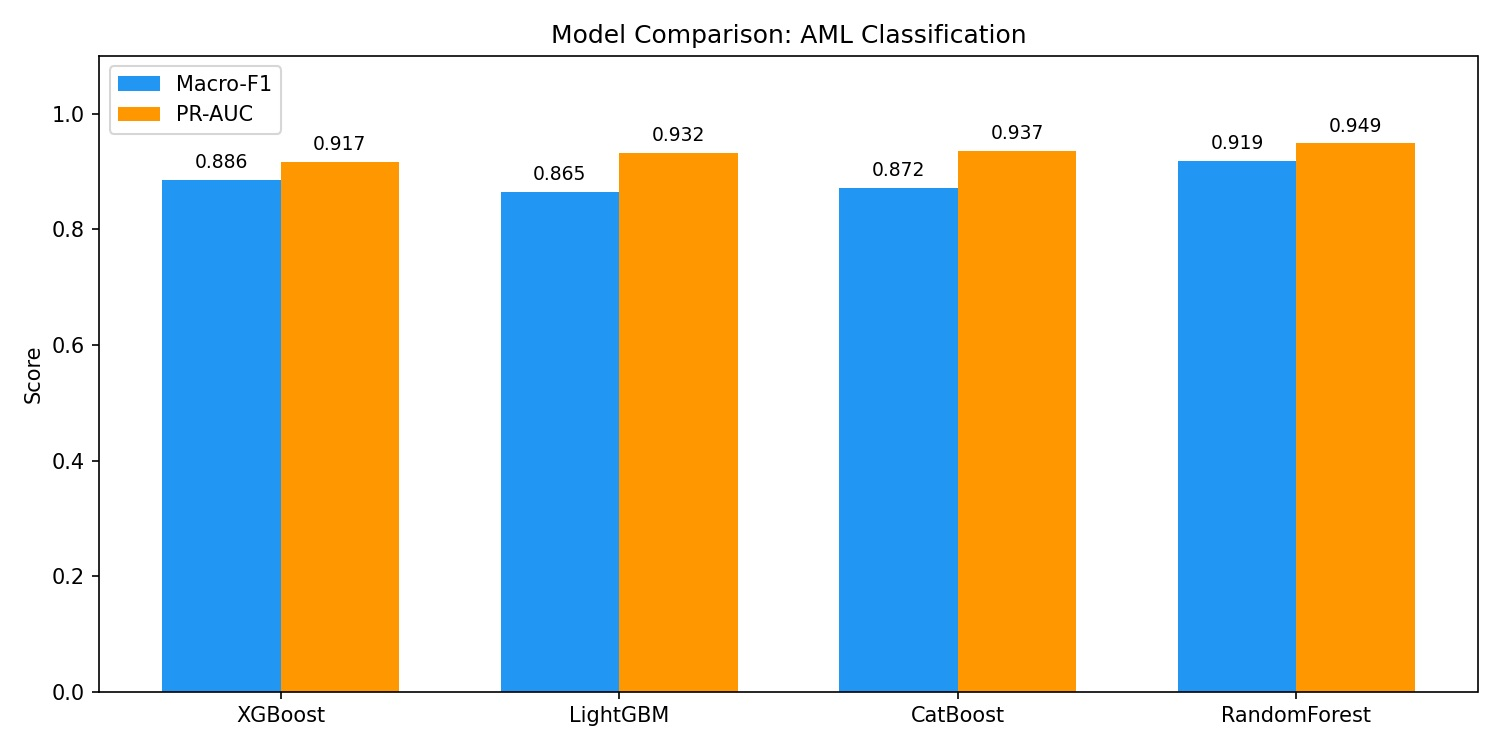
\includegraphics[width=0.85\textwidth]{figures/model_comparison}
    \caption{Model comparison: Macro-F1 and PR-AUC across four tree ensemble models.}
    \label{fig:model_comparison}
\end{figure}

\begin{table}[htbp]
\centering
\caption{5-Fold Stratified Cross Validation results for four tree ensemble models.}
\label{tab:model_results}
\small
\begin{tabular}{lccc}
\toprule
\textbf{Model} & \textbf{Macro-F1} & \textbf{PR-AUC} & \textbf{Accuracy} \\
\midrule
\textbf{RandomForest} & \textbf{0.919} & \textbf{0.949} & \textbf{0.927} \\
XGBoost & 0.886 & 0.917 & 0.900 \\
CatBoost & 0.872 & 0.937 & 0.887 \\
LightGBM & 0.865 & 0.932 & 0.880 \\
\bottomrule
\end{tabular}
\end{table}

\subsection{Confusion Matrix Analysis}

Figure~\ref{fig:confusion_matrix} shows the confusion matrix for the best model (RandomForest). The model achieves 95.9\% precision and 93.0\% recall for blocklisted detection, with only 4 false positives (normal addresses incorrectly flagged as blocklisted) and 7 false negatives. Given the small training set (150 samples vs.\ StableAML's 16,433), these results are encouraging.

\begin{figure}[htbp]
    \centering
    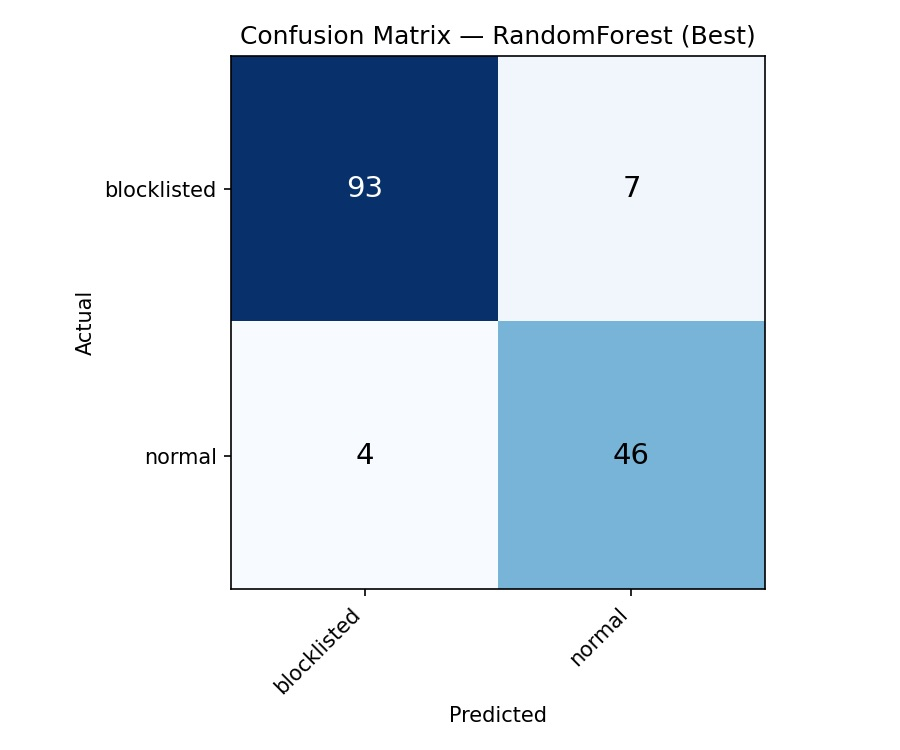
\includegraphics[width=0.55\textwidth]{figures/confusion_matrix}
    \caption{Confusion matrix for the best model (RandomForest). TN=93, FP=7, FN=4, TP=46.}
    \label{fig:confusion_matrix}
\end{figure}

\subsection{Feature Importance}

Figure~\ref{fig:importance_rf} shows the top 20 features by Mean Decrease Impurity (MDI) for RandomForest. The most discriminative feature is \texttt{drain\_ratio} (balance drain rate) --- blocklisted addresses have a mean of 0.21 vs.\ 1.37 for normal addresses, reflecting that frozen addresses cannot transfer funds out. Other top features include \texttt{out\_degree}, \texttt{sent\_count}, \texttt{unique\_receivers}, and \texttt{in\_out\_degree\_ratio}.

\begin{figure}[htbp]
    \centering
    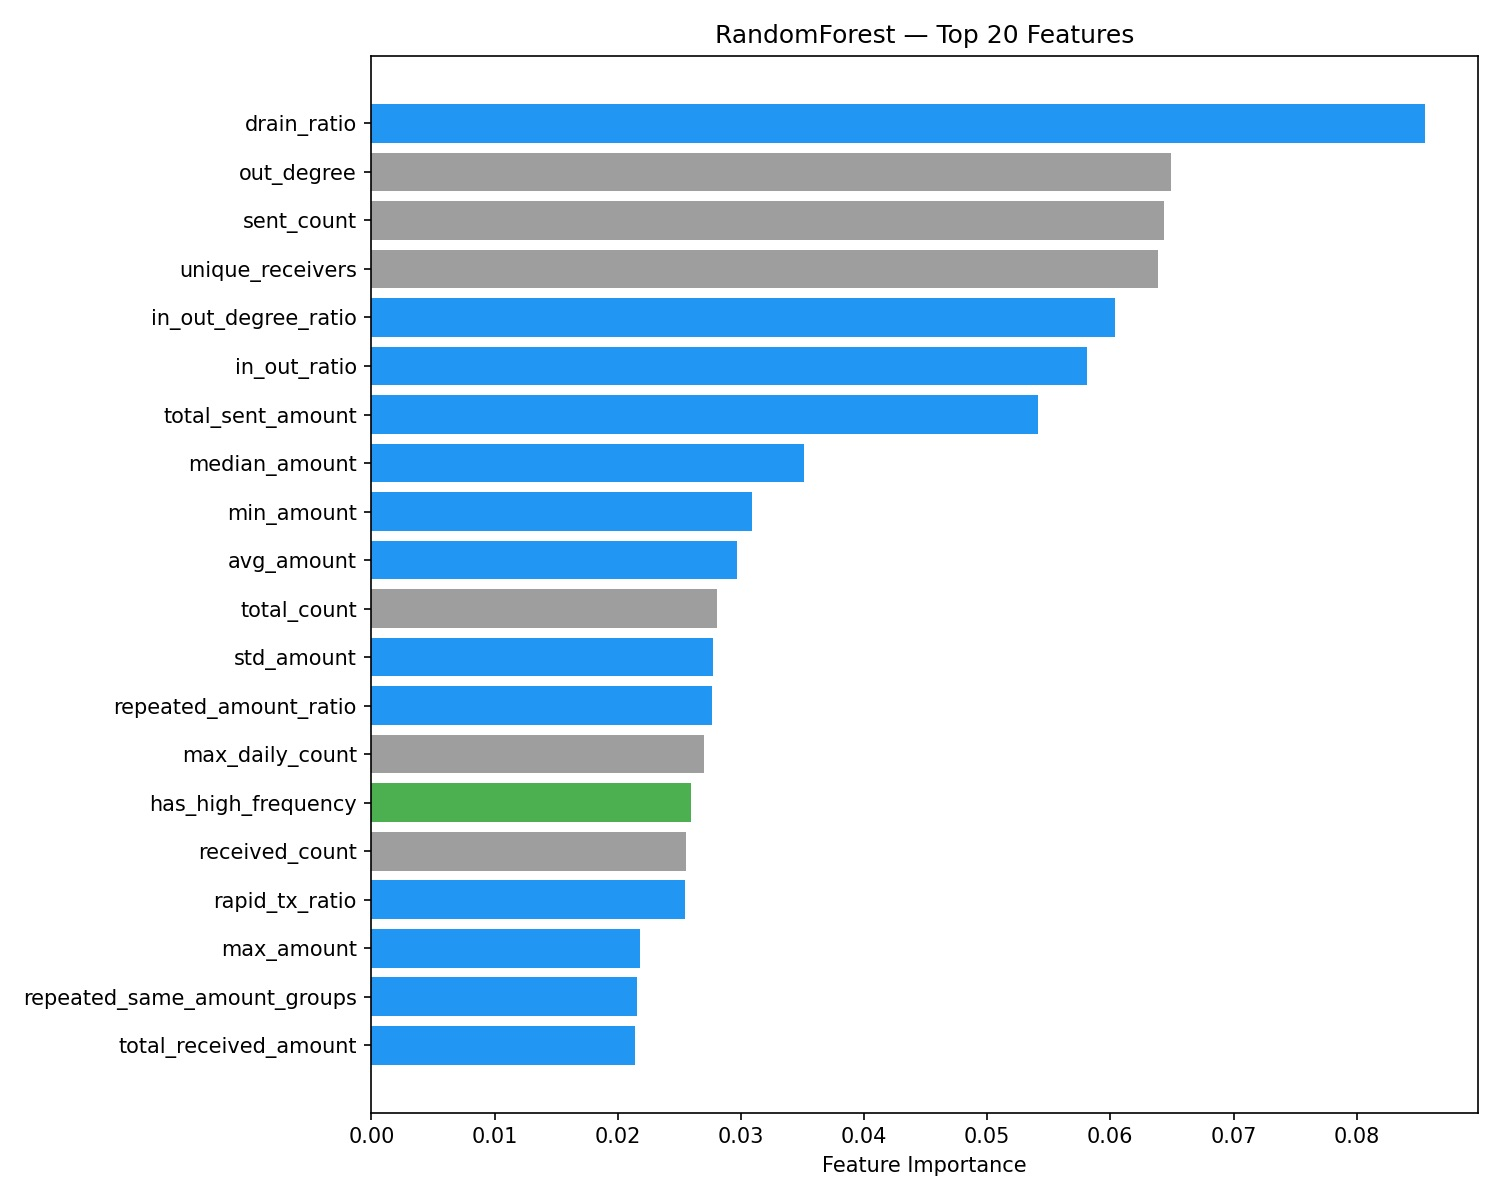
\includegraphics[width=0.85\textwidth]{figures/importance_randomforest}
    \caption{Top 20 feature importances (MDI) for the RandomForest model.}
    \label{fig:importance_rf}
\end{figure}

Figure~\ref{fig:importance_xgb} shows the feature importance for XGBoost (by Gain). The ranking differs: \texttt{total\_sent\_amount} and \texttt{counterparty\_flagged\_ratio} are the top two, reflecting that XGBoost leverages KYC label data and large transaction amounts more heavily than RandomForest.

\begin{figure}[htbp]
    \centering
    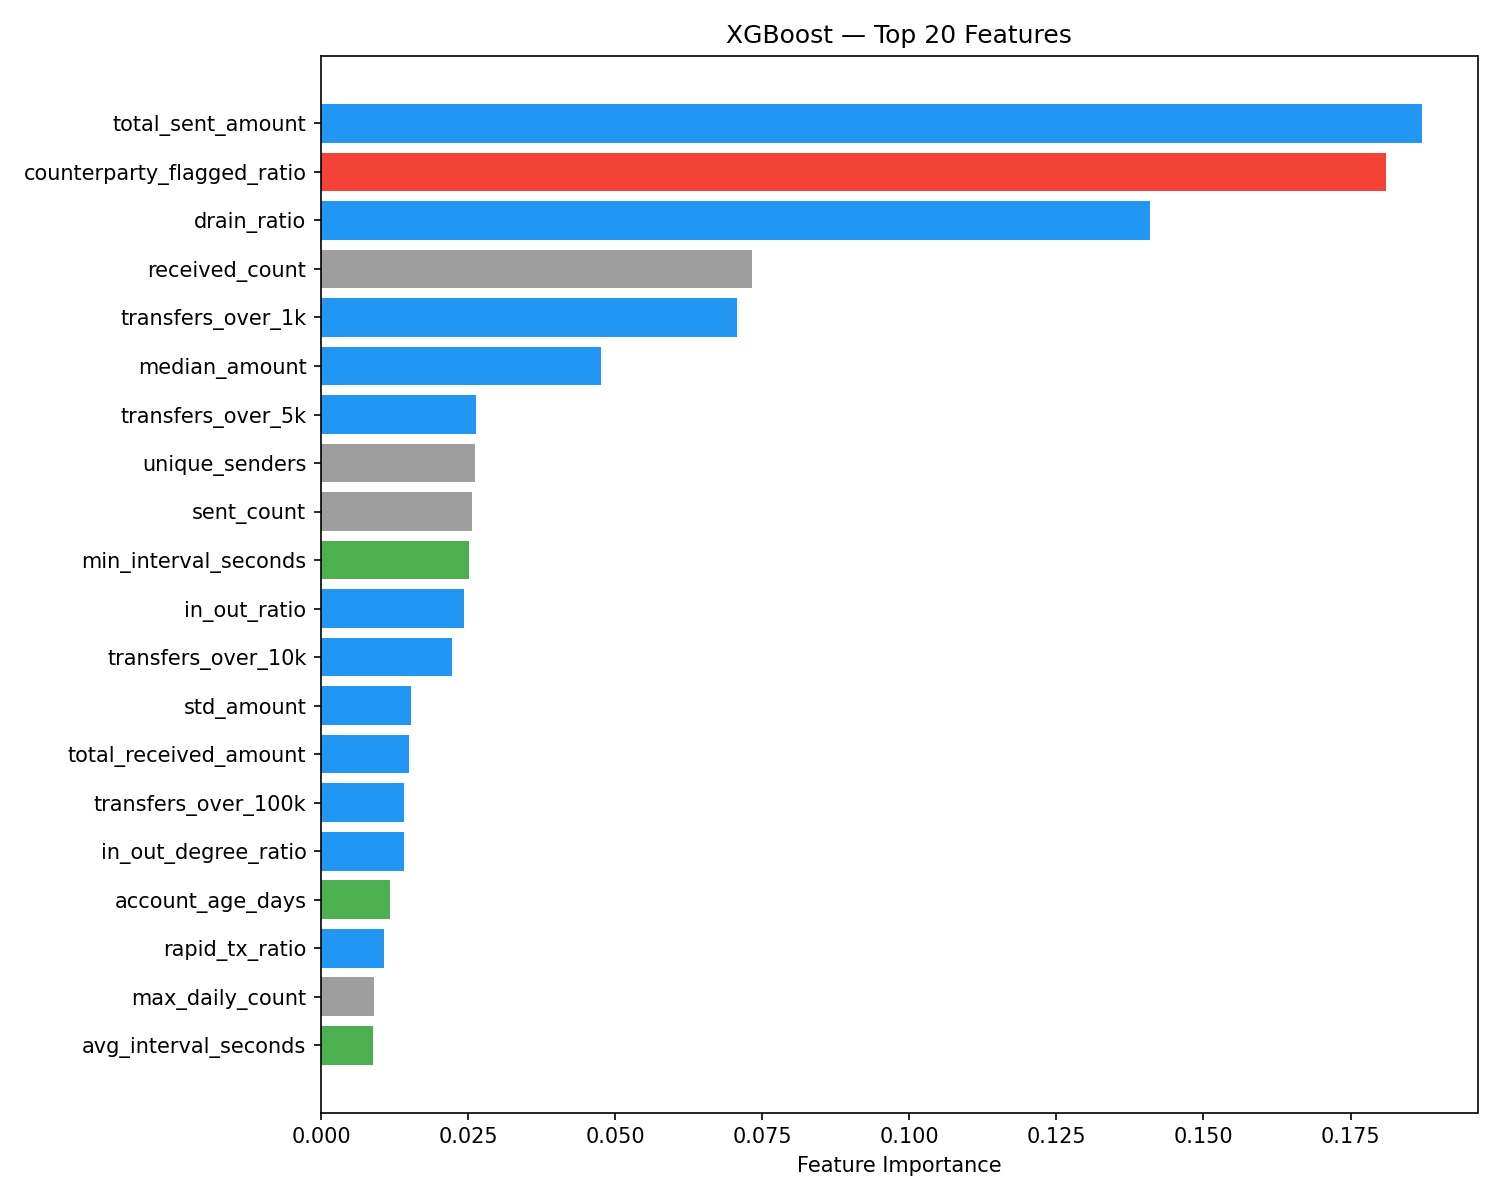
\includegraphics[width=0.85\textwidth]{figures/importance_xgboost}
    \caption{Top 20 feature importances (Gain) for the XGBoost model.}
    \label{fig:importance_xgb}
\end{figure}

\subsection{System Module Status}

\begin{table}[htbp]
\centering
\caption{Current implementation status of system modules.}
\label{tab:module_status}
\small
\begin{tabularx}{\textwidth}{l l X}
\toprule
\textbf{Module} & \textbf{Status} & \textbf{Description} \\
\midrule
\texttt{aml\_analyzer.py} & Implemented & Etherscan + TronScan API, blacklist (8,500+), bridge registry (20+), mixer (10), hybrid scoring \\
\texttt{trace\_graph.py} & Implemented & BFS tree, cross-chain resolution, adaptive depth, convergence tracking, Mermaid export \\
\texttt{ml/} pipeline & Implemented & Data collection, 61 features, 4 models trained, best model integrated \\
Bug fixes (P1--P5) & Implemented & Sampling bias and graph distortion corrections \\
\bottomrule
\end{tabularx}
\end{table}

\subsection{Known Limitations}

Five limitations are identified:
\begin{enumerate}
    \item \textbf{Limited data}: 150 samples is far fewer than StableAML's 16,433, and expanding the dataset is the most direct path to improved generalization.
    \item \textbf{Unverified Normal class}: randomly sampled ``normal'' addresses from the chain may include unlabeled laundering addresses (label noise), which could depress precision.
    \item \textbf{USDT/USDC only}: launderers who swap to ETH or other tokens via DEX protocols escape the current analysis scope entirely.
    \item \textbf{Real-time feature gap}: the ML scorer currently extracts features from the \texttt{RiskReport} object, which is a subset of the full behavioral profile; some temporal features require complete Transfer event data not available in the real-time scoring path.
    \item \textbf{Binary classification}: the current model only distinguishes blocklisted from normal, without finer sub-categories such as sanctioned, cybercrime, or terrorism financing.
\end{enumerate}


% =========================================================
\section{Milestones and Overall Schedule}
% =========================================================

\begin{table}[htbp]
\centering
\caption{Project milestones and schedule.}
\label{tab:milestones}
\small
\begin{tabular}{clp{8cm}}
\toprule
\textbf{Phase} & \textbf{Period} & \textbf{Milestone} \\
\midrule
1 & Weeks 1--3 (Done)  & Core system: \texttt{aml\_analyzer.py}, \texttt{trace\_graph.py}, registries \\
2 & Weeks 4--5 (Done)  & ML pipeline: data collection, features, training, integration \\
3 & Weeks 5--6 (Done)  & Bug fixes P1--P5, hybrid scoring, convergence tracking \\
4 & Weeks 7--9         & End-to-end validation; expand dataset to 1,000+ addresses \\
5 & Weeks 10--12       & Taint proportion analysis (FIFO/Haircut/Poison) \\
6 & Weeks 13--15       & Additional bridge support; performance benchmarks \\
7 & Weeks 16--18       & LLM explanation layer (exploratory); final report \\
\bottomrule
\end{tabular}
\end{table}


% =========================================================
\section{Work to Be Completed for the Next Report}
% =========================================================

\begin{itemize}
    \item \textbf{Dataset expansion}: Scale from 150 to 1,000+ labeled addresses with manual verification of the Normal class.
    \item \textbf{End-to-end validation}: Run the complete system on known laundering cases (Ronin Bridge, Harmony Bridge) to verify trace tree reconstruction.
    \item \textbf{OFAC SDN integration}: Supplement the blacklist with sanctioned addresses not covered by Tether's freeze list.
    \item \textbf{Additional bridge support}: Implement counterpart address resolution for Hop Protocol and Across Protocol.
    \item \textbf{Time window filtering}: Introduce configurable time windows to exclude ancient transactions that introduce false positives.
    \item \textbf{Taint proportion analysis}: Implement FIFO and Haircut methods to upgrade from binary risk to proportional confidence scoring.
    \item \textbf{LLM explanation layer} (exploratory): Prototype feeding JSON trace results into an LLM to generate natural language risk narratives, as validated by~\cite{watson2025} and~\cite{nicholls2024}.
\end{itemize}


% =========================================================
\addcontentsline{toc}{section}{References}
\printbibliography

\end{document}
